% !TEX encoding = MacOSRoman
\documentclass[handout]{beamer}
\usepackage[frenchb]{babel}
\usepackage[T1]{fontenc}
\usepackage[utf8]{inputenc}
\usepackage{graphicx}


% functions to plot
\def\func(#1){(#1)*(1-(#1))}
\hypersetup{colorlinks = true,linkcolor = blue,urlcolor  = blue}
            
\newcommand{\qGraph}[1]{\begin{center} \includegraphics[width =
\textwidth]{#1}\end{center}}

\newcommand{\mcl}{\mathcal}

\addtobeamertemplate{navigation symbols}{}{%
    \usebeamerfont{footline}%
    \usebeamercolor[fg]{footline}%
    \hspace{1em}%
    \insertframenumber/\inserttotalframenumber
}

\newenvironment{iPar}[1]{\textbf{#1} \begin{itemize}}{\end{itemize}}

\newcommand{\inc}{{inc}}
\newcommand{\cp}{{cmp}}
\newcommand{\bull}{$\bullet\;$} 

\newcommand{\esp}{\mathbf{E}} \newcommand{\ul}[1]{\underline{#1}}
\newcommand{\ol}[1]{\overline{#1}} \newcommand{\ora}[1]{\textbf{#1}}
\newcommand{\wh}{\widehat}
\newcommand{\mdp}{\medskip \pause}
\newcommand{\mc}{\mathcal}

\title{Consumer Choice under Risk}
\author{Microeconomics \\ 20851}
\date{}

\begin{document}

\frame{\titlepage}

\section[Outline]{}
\frame{\tableofcontents}

\section{}


\begin{frame}\frametitle{Roadmap}

\begin{iPar}{Up until now}
\item Consumer preferences
\item Consumer choice
\item Price and income effects
\end{iPar}\mdp

\begin{iPar}{This class: risk}
\item To understand insurance and investment decisions
\end{iPar}\mdp

\begin{iPar}{Coming up}
\item Intertemporal choice
\item Measuring welfare and well-being
\item Market equilibrium in an exchange situation
\item Production and strategic behaviour of firms
\item Auctions
\end{iPar}
\end{frame}

\section{Preferences}

\begin{frame}\frametitle{Preferences in an Uncertain Context}

\begin{iPar}{Generally speaking, people don't like risk}\item Average retirement income: \$$50 \; 000$/year \item  Imagine that you're saving for retirement:
You have to choose between (bonds, stocks ...) \item Problem
1: \begin{tabular}{ll} \textbf{asset without risk} & 50\; 000/an\\
\textbf{asset with risk} & 50\% chance  10 000/year \\ & 50\%  chance  90
000/year\end{tabular} \medskip \item Average income is 50 000/year in both cases, which one do you choose? \end{iPar}

\end{frame}

\begin{frame}\frametitle{Balancing Risk and Return}

\begin{iPar}{Three choice problems}
\item \begin{tabular}{lll} \textbf{Choice 1:} & \textbf{no risk} & 50\; 000/year\\
&\textbf{risk} & 50\% chance  10\; 000/year \\& & 50\%  chance  90\; 000/year\end{tabular} \mdp \item \begin{tabular}{lll}\textbf{Choice 2:} &  \textbf{no risk} & 50\; 000/year\\
& \textbf{risk} & 50\% chance  10\; 000/year \\ & & 50\%  chance  100\; 000/year\end{tabular} \mdp \item  \begin{tabular}{lll} \textbf{Choice 3:} & \textbf{no risk} & 50\; 000/year\\
& \textbf{risk} & 50\% chance  10\; 000/year \\ &&  50\%  chance
110\; 000/year\end{tabular} \end{iPar} \end{frame}


\begin{frame}\frametitle{The Expected Utility Approach}

\begin{iPar}{Lottery and expected utility} 
\item Lottery $\mathcal L = (p,X \;; 1-p,Y)$ : with
probability $p$ to get $X$, and probability $1-p$ to get $Y$ \item Expected utility $$
\mathbf \mathbb{E}_{{ \mathcal L}} (u) = p\times u(X) + (1-p) \times
u(Y)$$ \end{iPar}\mdp



\begin{iPar}{Preferences in lotteries} \item Model: Consumer prefers the
lottery $\mathcal L_1$ over the lottery $\mathcal L_2$ if $$\mathbf \mathbb
{E}_{{ \mathcal L_1}} (u) > \mathbf \mathbb{E}_{{ \mathcal L_2}} (u)$$
\item Note: Utility is cardinal (units and form matter). This is called the  \href{https://fr.wikipedia.org/wiki/John_von_Neumann}{von Neumann} and Morgenstern (vNM) utility. 
\end{iPar}

\end{frame}

\begin{frame}{Example}

\begin{iPar}{Context} \item $u(X) = \sqrt{X}$ \item $\mathcal L_1 =
(0.5,0\;; 0.5,16)$ et $\mathcal L_2 = (1,6)$ \item \textbf{Exercise A}: Expected return? \item
\textbf{Exercise B} What does the consumer choose?  \item \textbf{Exercise C}: Does the utility function $u(X) = X$ result in the same behaviour?\end{iPar}

\end{frame}

\begin{frame}{Identifying preferences from choices}

\begin{iPar}{Preferences do not vary with affine transformations}
\item Affine transformation: $\wh u = a u +b$ with $a>0$
\begin{align*}
\esp_{L_1} \wh u \geq \esp_{L_2} \wh u & \iff  a\esp_{L_1} u + b \geq a\esp_{L_2} u + b \\ & \iff 
 \esp_{L_1} u  \geq \esp_{L_2} u
\end{align*}\mdp

\end{iPar}

\end{frame}

\section{Risk Aversion and Risk Seeking}

\begin{frame}\frametitle{Risk-Averse and Risk-Seeking Consumers}
\begin{iPar}{Different attitudes towards risk} \item Risk aversion: consider $L = (p, X\;; 1-p,Y)$\\
If we denote $Z = p X + (1-p)Y $. \mdp

consumer is risk-averse if he prefers $\mathcal L' = (1,Z)$ over $\mathcal L$  \mdp \item Risk-seeking: he prefers $ \mathcal L = (p, X\;; 1-p,Y) $ over $\mathcal L' =
(1,Z)$ \end{iPar}\mdp

\begin{iPar}{What do we observe?} \item There is some risk-seeking behaviour (casinos
... ) but it doesn't take into account the value of the "experience" \item  A lot of risk aversion (insurance, saving, investment ...) \end{iPar} \end{frame}


\begin{frame}\frametitle{Risk Aversion and Concavity of the Utility}

\begin{iPar}{Risk aversion} \item Consumer with utility $u$ \item Given
$(X,Y)$ and $p$, define  $z \equiv pX + (1-p)Y $ \item Risk-aversion implies: $ u(Z) \geq pu(X) + (1-p)u(Y)$ \item This is the equivalent of saying that $u$ is concave. \end{iPar}\mdp

\begin{iPar}{Risk-neutrality}
\item Indifference between $$ \mathcal L = (p, X\;; 1-p,Y) \quad and \quad  \mathcal L' = (1,Z)$$
\item Corresponds to linear utility $u(X) = a X + b$, in particular $u(x) = x$.
\end{iPar}

\end{frame}

\begin{frame}{Measuring risk aversion}


\begin{figure}
\centering
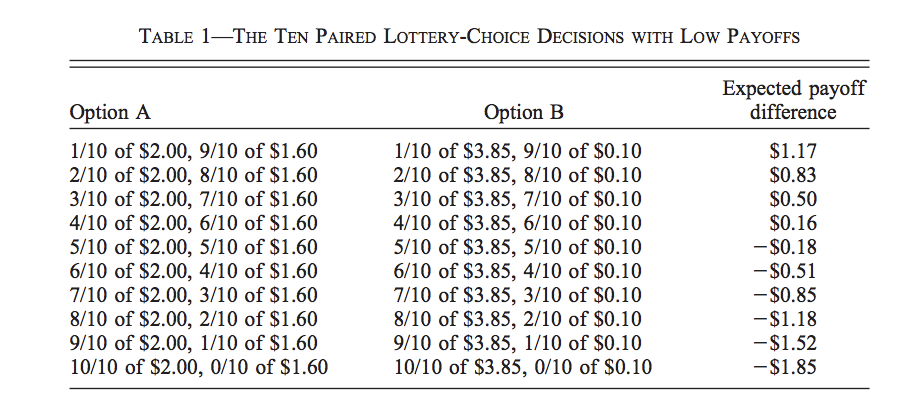
\includegraphics[scale=0.4]{lotteries.png} 
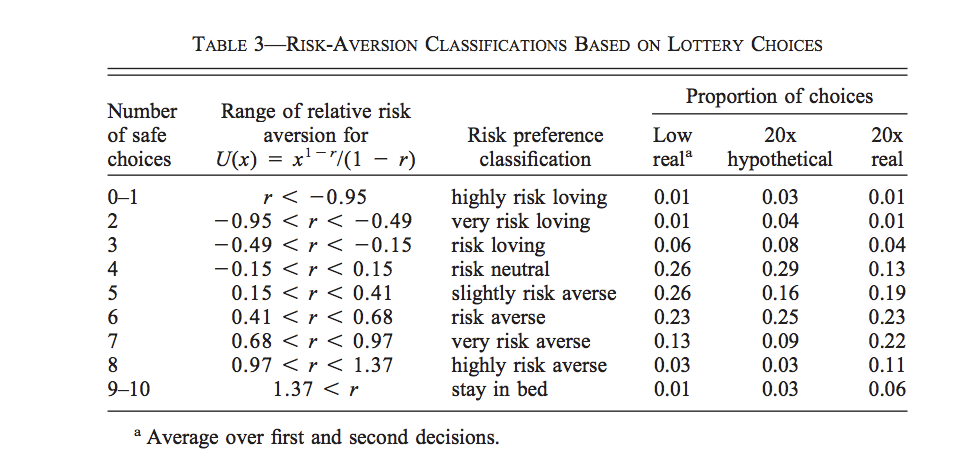
\includegraphics[scale=0.4]{choices.png}
\caption{\href{https://pubs.aeaweb.org/doi/pdfplus/10.1257/000282802762024700}{Holt et Laury (2002), American Economic Review}}
\end{figure}

\textbf{Exercise D}: Why does a risk-averse agent wait longer in the Holt and Laury experiment?
\end{frame}

\section{Risk Premium}

\begin{frame}\frametitle{Risk Premium}

\begin{iPar}{Definition} \item Consider the lottery $\mc L =
(p,X\;;1-p,Y)$. Define $Z$ as $Z \equiv pX+ (1-p)Y$. \item Find $Z'$ such that $u(Z') = pu(X) + (1-p)u(Y)$ \item $Z'$ is a certain equivalent of $\mc L$ \item When risk-averse, $Z' < Z$ and $
\pi = Z-Z'$ is the risk premium \item The risk premium is the amount equal to the gain/loss provided by the lottery \item It's how much we should give the consumer to entice him to take the risk (compensation). Or, how much he is willing to pay to eliminate of a risk. 
\item This is used to evaluate risky assets and demand for insurance. 
\end{iPar}

\end{frame}

\begin{frame}{Example}
\textbf{Exercise E}: An agent has the utility function $u(X)=\ln X$. His initial wealth is $X_0 = 100$ and he's facing the risk of losing 50 with probability 0.5 and win 50 with probability 0.5. What is the maximum amount he's willing to pay to avoid that risk? \\
\textbf{Exercise F}: With $u(X) = \sqrt X $, is the risk premium smaller?
\end{frame}


\section{Applications: Insurance and Investment}

\begin{frame}\frametitle{Several goods we buy are lotteries}
\begin{iPar}{Financial assets, insurance, investment goods ...
almost everything} \item Stocks (yields 10 if the firm performs well, yields 0 if she underperforms) \item Fire insurance (yields 5 if house burns down, yields 0 otherwise) \item Used car (value of 3 if good quality, value of 0 if lemon) \item
Starting a business (yields 15 if it works , -5 if it fails) \item Getting married, choosing a career, getting surgery, driving a vehicle... all of these are choices in a risky context. \end{iPar} \mdp \textbf{Later:} practical implications of risk-aversion \end{frame}

\begin{frame}\frametitle{Insurance and Co-insurance -- I}
\begin{iPar}{Context: two consumers facing risk}  \item Each is employed with a 50\% probability, income 100 \item Unemployed (U) with a 50\% probability, income 0\end{iPar}\mdp

\begin{iPar}{Employment insurance} \item An insurance program where instead of the consumer 1 getting $I_1$ and the consumer 2 getting $I_2$ they both get $(I_1+I_2)/2$ regardless of their employment status \end{iPar}

\end{frame}

\begin{frame} \frametitle{Insurance and Co-insurance -- II}

\begin{iPar}{Insurance is beneficial} \item Without insurance: 50\%
of getting 0, 50\% of getting 100 \item expected utility $ .5 [u(0) + u(100)] $ \item
With insurance 25 \% of getting 0, 25\% of getting 50, 25\% of getting 50, 25\% of getting
100 \item expected utility $.25[u(0) + u(50) + u(50) + u(100)]$ \item
Insurance is beneficial if and only if \begin{eqnarray*} & .25[u(0) + u(50) +
u(50) + u(100)] > .5 [u(0) + u(100)]\\ \iff& u(50) > .5[u(0)+u(100)]
\end{eqnarray*}\item True if they are risk-averse  \end{iPar}

\end{frame}

\begin{frame} \frametitle{Insurance and Co-insurance -- III}
\begin{iPar}{In practice} \item The issue of doing it informally:
ex-ante (before knowing the outcome) we want insurance (sharing), but ex-post, if employed, we don't want to share our income \item That is where insurance companies come in
(making sure people pay even though they got lucky)\end{iPar}

\end{frame}

\begin{frame} \frametitle{The Law of Large Numbers and Insurance}

\begin{iPar}{Law of large numbers} \item Consider a random variable $Z$
equal to $X$ with probability $p$ and $Y$ with probability $1-p$ \item If $Z_1,
\cdots , Z_n$ are independent with the same distribution $(p,X \;; 1-p,Y)$
Then $$si\; N \to +\infty,\quad  \frac{1}{N} (Z_1 + Z_2 + \cdots + Z_n)
\to pX + (1-p)Y$$

\item The empirical average converges towards the expected value \end{iPar}
\end{frame}


\begin{frame} \frametitle{The Law of Large Numbers and Insurance}

\begin{iPar}{What this means for insurance} \item When several individuals are sharing risk, and their risks are independent, then everyone recieves exactly their expected income \item If individuals are risk-averse, this result is good \item The larger the number of indivuals sharing risk is, the higher their well-being will be  \end{iPar}

\end{frame}

\begin{frame}\frametitle{Insurance is Important: An Investment Example}
\textbf{Investment project}\begin{itemize} \item An individual has a wealth of 9 and can decide to do nothing or to use all his wealth to start a business corresponding to the lottery $\mc L = (.5,0 \;; .5,25)$ \item Utility $u(X) = \sqrt{X}$ \item \textbf{Exercise G}: What is the expected return? What will he choose ? \end{itemize}\end{frame}

\begin{frame}\frametitle{Insurance Encourages Investment}

\begin{iPar}{With insurance} \item Instead of investing alone, the entrepreneur can get financing from an angel investor who will provide half the capital and recieve half the return \item The entrepreneur gets to keep 4.5 and gets half of the return \item The lottery is now $\mc L' = (.5,4.5 \;; .5,17)$ \item \textbf{Exercise H}: What will he choose?\end{iPar}

 \end{frame}

\section{Criticism of Expected Utility}



\begin{frame}{Criticism of Expected Utility}
\begin{itemize}
\item Allais' Paradox
\item Ellsberg's Paradox
\item Kahneman and Tversky
\end{itemize}
\end{frame}


\begin{frame}{Choice}


We draw a number between 0 and 99 with probability 1/100 of drawing each integer: 

\begin{table}[H]
\begin{tabular}{lrrr}
\hline \hline
Lotteries & 0 & 1-10 & 11-99 \\
$L_1$ & 50 & 50 & 50 \\
$L_2$ & 0 & 250 & 50 \\
\hline \hline 
\end{tabular}
\end{table} 


\end{frame}

\begin{frame}{Choice}

Now, let's choose again between

\begin{table}[H]
\begin{tabular}{lrrr}
\hline \hline
Lotteries & 0 & 1-10 & 11-99 \\
$L_3$ & 50 & 50 & 0 \\
$L_4$ & 0 & 250 & 0 \\
\hline \hline 
\end{tabular}
\end{table} 

\end{frame}

\begin{frame}{Maurice Allais and his Paradox}

\textbf{Exercise I}: Show that $L_1 \succ L_2$ and $L_4 \succ L_3$ are incoherent with the expected utility theory. 

\begin{figure}
\centering
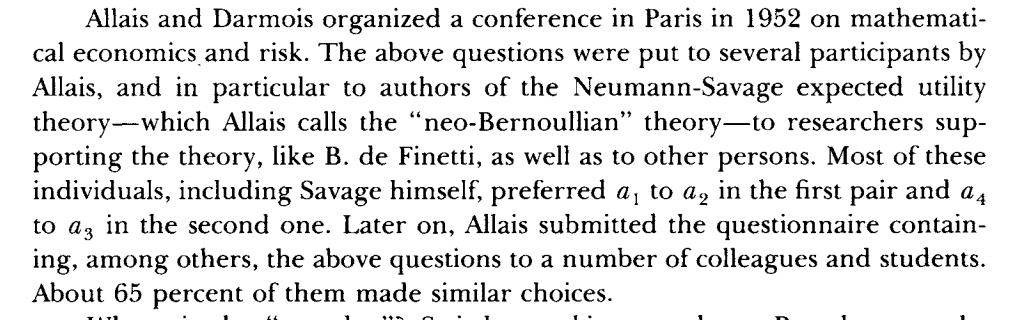
\includegraphics[scale=0.5]{allais.png}
\caption{\href{https://pubs.aeaweb.org/doi/pdf/10.1257/jep.5.2.179}{Munier 1991, Journal of Economic Perspectives}}
\end{figure}

\end{frame}

\begin{frame}{Choice}

An urn contains 90 marbles. 30 are red. The other 60 are either black or white. The proportion of black and white marbles is unknown. 
Choose between
\begin{table}[H]
\begin{tabular}{lrrr}
\hline \hline
Lotteries & red & black & white \\
$L_1$ & 50 & 0 & 0 \\
$L_2$ & 0 & 50 & 0 \\
\hline \hline 
\end{tabular}
\end{table} 

\end{frame}

\begin{frame}{Choice}

An urn contains 90 marbles. 30 are red. The other 60 are either black or white. The proportion of black and white marbles is unknown.

\begin{table}[H]
\begin{tabular}{lrrr}
\hline \hline
Lotteries & red & black & white \\
$L_3$ & 50 & 0 & 50 \\
$L_4$ & 0 & 50 & 50 \\
\hline \hline 
\end{tabular}
\end{table} 
\pause

\end{frame}

\begin{frame}{Ellsberg's Paradox}

\textbf{Exercise J} Show that the combination of $L_1 \succ L_2$ and $L_4 \succ L_3$ does not respect the expected utility for any subjective probability of black marbles. 

\href{https://fr.wikipedia.org/wiki/Daniel_Ellsberg}{Pentagon Papers}

\end{frame}

\begin{frame}{Kahneman and Tversky: Perspective Theory}

Imagine a new disease expected to kill 600. Two programs proposed. 

\begin{itemize}
\item (Positive Framing): A) 200 saved, B) 1/3 probability that 600 saved, 2/3 that none saved
\item (Negative Framing): C) 400 will die, D) 1/3 nobody dies, 2/3 all die
	\end{itemize}


If this interests you, read: \href{https://www.uzh.ch/cmsssl/suz/dam/jcr:00000000-64a0-5b1c-0000-00003b7ec704/10.05-kahneman-tversky-79.pdf}{Khaneman et Tversky (1979)}

\end{frame}

\end{document}




